\documentclass[a4,11pt]{report}

\usepackage[pdftex]{graphicx}
\usepackage{setspace}
%\usepackage{lineno}
\usepackage{color}
\usepackage{float}
\usepackage{enumitem}
\definecolor{PiranaOrange}{rgb}{0.9,0.4,0.1}
\definecolor{Blue}{rgb}{0.0,0.0,0.7}
\definecolor{Red}{rgb}{0.7,0.0,0.0}
\definecolor{Grey}{rgb}{0.4,0.4,0.4}
\definecolor{lightGrey}{rgb}{0.9,0.9,0.9}

\bibliographystyle{unsrt}
\usepackage{listings}
\lstset{basicstyle=\small\ttfamily,breaklines=true,backgroundcolor=\color{lightGrey}}

\renewcommand{\familydefault}{\sfdefault}

\oddsidemargin 1.5cm

\textwidth 14cm

\begin{document}


\title{
  \vspace{-100pt}
  \textbf{
    \textcolor{PiranaOrange}{\Large Pirana}
  }\\
  \vspace{5pt}
  \scriptsize \textcolor{Grey}{The pharmacometrician's workbench} \\
  \normalsize
  \vspace{15pt}
  \hspace{15pt}
\includegraphics[scale=0.2]{../images/pirana_logo.jpg}\\
  \vspace{15pt}
  \scriptsize Version $\geq$ 2.9.7\\Pirana on Metworx user guide \\
  \vspace{5pt}
  \scriptsize {\today} \\
  \date{}
}
\maketitle

\section*{Introduction}\label{introduction}

Pirana, a modeling interface for NONMEM and PsN, is by default installed
on Metworx 3 instances. This document is an overview of how to get started with Pirana on Metworx, as
there are a few noteworthy differences compared to running Pirana on
your desktop computer. We also provide some additional tips and tricks.
A full user manual of Pirana is available at
\href{www.pirana-software.com}.

\vspace{10pt}

\noindent\emph{This guide will be updated at regular intervals, and is
available online from www.pirana-software.com/\#docs. This document
assumes Pirana 2.9.7 or up, and Metworx version 3.0 or up.}

\section*{License file}\label{license-file}

The license file for Pirana is commonly not included on the Metworx
instance, and therefore it has to be added by each individual Metworx user.
Please note that without a license file, you can still access and use
Pirana, but you will see a popup screen come up regularly asking for the
license file. If you have a license file for Pirana, you can either
upload the file manually to \texttt{/data} to activate Pirana, or from
within Pirana go to ``Help'' $\rightarrow$ ``Install license file''
and select the file from a location within Metworx. If you do not have a
license file yet, please contact \texttt{info@pirana-software.com} to
obtain one or request further info.

\section*{Home folder / settings}\label{home-folder-settings}

Please keep in mind that the Metworx workflow is reprovisioned each time
a new workflow is started. This means that all folders that are not in a
persistently location -- e.g.~your home folder -- will be wiped when the
workflow is destroyed. Your persistent data storage in Metworx is
available in the folder \texttt{/data}, which will also be used by Pirana to
store some preferences.

\vspace{10pt}

\noindent\scriptsize{\textcolor{Blue}{Note:} \textcolor{Grey}{Pirana normally stores all user
settings (such as UI settings, a list of projects, software settings
etc) in your home folder, in \texttt{\textasciitilde{}/.pirana} to be
specific. To allow you to persist your preferences and
projects between Metworx workflows, Pirana will use \texttt{/data} to store these settings.}}\normalsize

\section*{R libraries}\label{r-libraries}

A commonly used selection of R libraries is installed by default in
Metworx, but other libraries will have to be installed manually. Since
obviously we do not want to re-install the same R libraries each time we
start a new Metworx workflow, these libraries should also be installed
into the persistent folder, in \texttt{/data/R/lib} to be precise.
This is the folder that is automatically picked up by both RStudio and
Pirana as the default location for custom R libraries. Therefore, when
installing a custom R library for use within RStudio or Pirana, use
e.g.~the command:

\begin{verbatim}
 install.packages("ggplot2", library="/data/R/lib")
\end{verbatim}

or, when installing from GitHub:

\begin{verbatim}
 install_github("hadley/ggplot2", library="/data/R/lib")
\end{verbatim}

When running R scripts included with Pirana, you might encounter an
error that a library was not found (e.g. \texttt{xpose4}). When such an
error occurs, use the above syntax to install the missing library into
the persistent R libraries folder \texttt{/data/R/lib}.

\section*{Parallelization}\label{parallelization}

Pirana can instruct PsN to run NONMEM models on the Metworx cluster formed by the computational nodes that you started.
Keep in mind that there are basically two ways of running in parallel that need to be distinguished:

\begin{itemize}

\item{\textit{Running a single model in parallel over multiple
computational cores (using MPI and SGE)}}

To use this approach, several arguments need to be specified with the \texttt{execute}
command. These arguments are already built into Pirana for Metworx and
the job scheduler is also set by default to SGE. So to run a single
model over multiple cores, you only have to select \textbf{auto-MPI} and
select the number of cores you want to use. You can check in the
\textbf{Cluster monitor} in Pirana that the model is actually distributed onto the computation
server.

\begin{figure}[H]
\centering
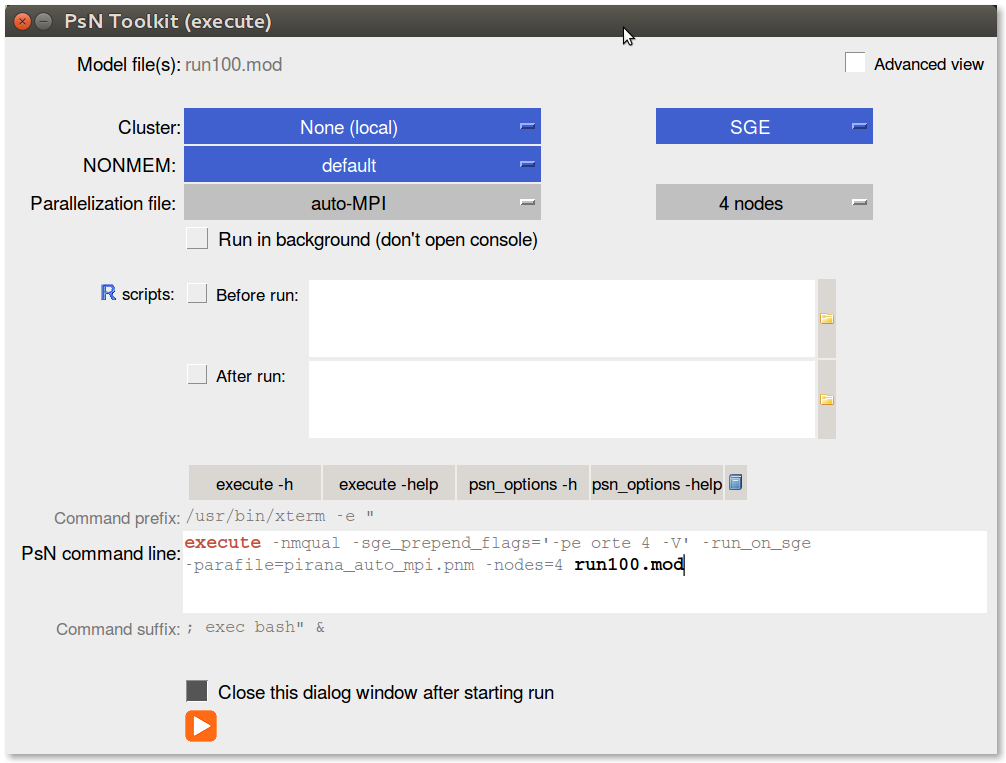
\includegraphics[scale=0.25]{pirana1.png}
\caption{Screenshot 1}
\end{figure}

\item{\textit{Running several models in parallel, e.g. bootstrap}}

In this case we usually don't want to use MPI-paralellization, so we set the \textit{parallelization file} to \textbf{off},
but keep the \textit{job scheduler} \textbf{SGE} selected. This will distribute the runs to the cluster, but won't split single runs over multiple cores.
An example is given below.

\begin{figure}[H]
\centering
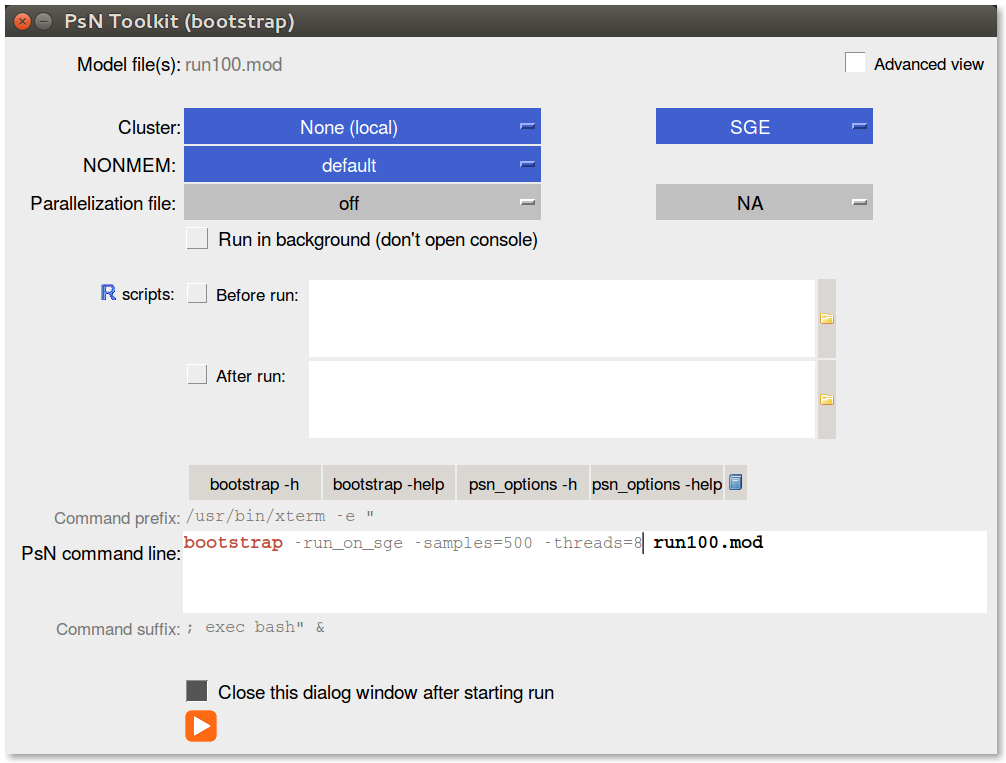
\includegraphics[scale=0.25]{pirana4.png}
\caption{Screenshot 1}
\end{figure}

\end{itemize}

\noindent\scriptsize{\textcolor{Blue}{Note:} \textcolor{Grey}{Please refer to the manuals for PsN and NONMEM for more information on
parallelization with job schedulers (SGE in this case) and MPI.}\normalsize

\vspace{10pt}

\noindent Anytime you run models using SGE, they will run on the computational node(s) that were started in the Metworx workflow.
You should be able to see those runs in the tabs \textbf{Runnning}, \textbf{Scheduled}, or
\textbf{Finished} in the cluster monitor within Pirana. See Pirana manual for more details on the cluster monitor.

\end{document}
